% !TeX spellcheck = en_GB
%pc version
\documentclass[11pt, a4paper, oneside, openright]{book}
%print version
%\documentclass[11pt, a4paper, hidelinks, twoside, openright]{book}
%\usepackage[bindingoffset=20mm]{geometry}

\usepackage[english]{babel}

\usepackage[style=apa, sortcites=true, sorting=ynt, maxalphanames=2,maxbibnames=99,natbib=true]{biblatex}

\bibliography{biblio.bib}

\usepackage{hyperref}
\hypersetup{hidelinks}

\usepackage{caption}
\captionsetup[figure]{font=small,labelfont=small}

\usepackage{csquotes}

\usepackage{graphicx}

\usepackage{amsfonts}
\usepackage{amsmath}
\newtheorem{definition}{Definition}
\newtheorem{hypothesis}{Hypothesis}
\DeclareMathOperator*{\argmax}{arg\,max}
\DeclareMathOperator*{\argmin}{arg\,min}

\usepackage{unicode-math}
%\setmathfont{TeX Gyre Termes Math}
\defaultfontfeatures{Ligatures=TeX}

\usepackage{etoolbox}

\makeatletter 
\let\c@table\c@figure
\let\c@lstlisting\c@figure
\makeatother

%\usepackage[bottom, hang]{footmisc}

%\usepackage{booktabs}
%\usepackage{array, longtable}


\title{Topic Models}
\author{Michele Ciruzzi & Carlo Debernardi}

\begin{document}

\maketitle

LICENSE CC-BY 4.0 \\

\includegraphics{fig/cc-by}\\
Source code available online at \url{https://github.com/TopicModels/topicmodels.github.io}
\clearpage

\tableofcontents
%\listoftables
%\listoffigures

\chapter{Definitions}

We start by defining the object of our interest: a (textual) document.
\begin{definition}[Document]
	\label{def:doc}
	A document $d$ is an ordered set of $\Omega_d$ words with repetitions. \\
	We can formally write $d = \{{\omega_d}_i\}_{i=1..\Omega_d}$
\end{definition}
This definition does not depend on the mathematical nature of words, which can be in fact actual words or even, for example, words and punctuation or DNA triplets. The only important thing is that the words belong to the same set. \\
Similarly, we can define a corpus:
\begin{definition}[Corpus]
	A corpus $\Gamma$ is a set of $D$ documents. \\
	We can formally write $\Gamma = \{d_i\}_{i=1..D}$
\end{definition}

The next step is the important one: what is a Topic Model?
Qualitatively, a Topic Model is a set of rules that classifies each document by the topic dealt with in it.
Generally speaking, a model gives predictions with a certain degree of confidence. 
So, we expect that a Topic Model does not provide a unique matching between a document and a label, but, rather, that it provides a measure of the confidence for each matching, or equivalently a description of the mix of topics dealt with within each document.
In other words, a Topic Model classifies the documents of a corpus in $K$ groups (called \textbf{topics}) by giving a score to each couple composed by a document $d$ and a topic $k$ which expresses the degree of confidence of the model in classifying the document $d$ in the topic $k$.
For clarity, we will call $\mathcal{K}$ the set of the $K$ topics.
\begin{definition}[Topic Model]
	\label{def:tm}
	A Topic Model is a function $s: \Gamma \rightarrow {\mathbb{R}^+}^K$ which maps each document of the corpus to a vector of scores, one for each topic. The score is increasing in the confidence of the model in classifying a document in each topic.
\end{definition}
This definition is very general and somehow obscure, but it will become more clear when the algorithms to infer Topic Models will be introduced.

Another flaw of this definition is the difficulty in interpreting the values of the scores. What do the scores represent? How can we compare the scores among the documents of the corpus?
We notice that if we normalize the score vector using a 1-norm (i.e. the sum of the values) we in fact project the vector to the K-1 simplex, which can be interpreted as a probability distribution, or as a distribution of topics inside documents.
\begin{definition}[Normalized Topic Model]
	A normalized Topic Model is a function $\tilde{s}: \Gamma \rightarrow {\Delta}^{K-1}$ which gives the probability for each document to be classified in a topic. Additionally, we have $\mathbb{P}(d|k) = \tilde{s}_k(d) = \frac{s_k(d)}{\|s(d)\|_1}$ for $k \in \mathcal{K}$.
\end{definition}
Hereinafter, unless otherwise specified, when we will refer to a Topic Model we, in fact, will indicate a normalized Topic Model.

Finally, $K$ remains to be discusses. We have introduced the number of topics without specifying how to determine it. This is because we can divide Topic Model algorithms in two groups: \textbf{parametric} and \textbf{non-parametric} ones.
A non-parametric algorithm is able to infer not only the model but also the number of topics, while a parametric one needs the number of topics to be fixed \textit{a priori} to be fully defined, and it does not exist any general rule to fix $K$.

\chapter{From words to vectors}
The definition of document~\ref{def:doc} is accurate and conveys all the available information, but it gives us a mathematical object (an ordered set) which is generally difficult to manage because it does not abstract (and so simplify) the problem, like a 1:1 map\footnote{On the relative uselessness of too accurate representations there are two short essays by J.L. Borges (``Del rigor en la ciencia'' in \textit{``Historia universal de la infamia''}) and U. Eco (``Dell'impossibilità di costruire la carta dell'impero 1 a 1'' in \textit{``Il secondo diario minimo''})}.

The problems of such an accurate description are mainly two: computationally, we have no possibility to compress data, and so our analysis will be strongly limited by the computational resources we have available, thus preventing an application to large corpora; mathematically, we have too much information to be accounted for in the model, which strongly limits the formal tools we can use.

In this chapter we describe which hypotheses and methods are adopted in the context of the Topic Model algorithms, in order to get a more manageable representation of our data.

\section{Bag-of-Words and n-grams}
\label{sec:bow}
The goal of each Topic Model algorithm is to regroup documents which deal with the same topic.
All the algorithms we will present in the following sections share some common hypotheses.
\begin{hypothesis}
	\label{hyp:topic}
	A topic can be effectively characterized by the words used to talk about it.
\end{hypothesis}
With this hypothesis we are assuming that when we switch topic in a text, the most significant change we make is the lexical one. Of course it will not be the only change we make, for example we can also change the average length of sentences, but this hypothesis states that this is the most important one.
\begin{hypothesis}[Bag-of-Words]
	We can describe a document as an \textit{unordered} set of words with repetitions without losing too much information.
\end{hypothesis}
Given the hypothesis~\ref{hyp:topic} it is natural to focus our attention more on the lexicon used in the documents than on the syntax. The Bag-of-Words hypothesis does exactly this: it states that the most important thing in a corpus to infer a Topic Model (and so the only one we have to care about in the algorithms) is the frequency of the words contained in the documents and not their order.

Sometimes this hypothesis is too strong, and we hypothesize that the order of the words is also locally (i.e. in a neighbourhood of each word in the ordered set) important, because the few words that precede or follow a word are important to specify the context, and so the meaning.

To recover the information brought by (local) order there are two possibilities: to abandon the Topic Model setting in favour of graphical models \parencite[e.g.][]{kang2018}, however they are computationally very expensive, or to adopt the \textit{n-grams} representation.
\begin{definition}[N-grams representation]
	Given a document $d$ its n-grams representation is the ordered set with repetitions of the n-uple of consecutive words. We can express the n-grams representation $\gamma_n(d) = \{\{\omega_i\}_{j..j+n-1}\}_{1..\Omega_d-n+1}$.
\end{definition}
It is immediately evident that $d = \gamma_1(d)$ if we consider a 1-uple equivalent to the single element that composes it. Moreover we can extend the Bag-of-Words hypothesis to a new Bag-of-n-grams one, where the order is important inside each n-uple but not among them.

It is very common that when a n-gram representation is used, a range for n is considered: in practice both single words and 2-grams (bigrams) and eventually 3-grams (trigrams) are simultaneously considered as input for the algorithms. Formally we can express this idea as $\gamma_{1..n}(d) = \cup_{i=1}^n \gamma_i(d)$.

\section{Preprocessing}
Preprocessing is the totality of the actions performed to transform the available sources of data, for example websites or paper documents, into a format which can be used as input for a Topic Model algorithm.

In this section we will not discuss the technical preprocessing required to transform data sources in a machine-readable set of words; instead, it is common to adopt some techniques to clean the data before passing them to an algorithm.
There are a practical and a theoretical reason to do this: removing some uninteresting words from a document reduces the memory requirements to process the data, allowing for processing larger corpora; given the hypothesis~\ref{hyp:topic} we can assume that certain words are not indicative of any topic (like pronouns, to be and to have verbs, conjunctions, etc.) or that they are not statistically significant because they are too much or too little frequent.\\
We will define some transformations which generally redefine the set of words $\Omega = \{{\omega_d}_i 	; \forall d,i\}$ and transform a document by mapping a subset of words from the original set $\Omega$ to a new set $\mathcal{W}$.

\subsection{Stopwords}
\label{sec:sw}
To reduce the dimensionality of the dataset and, hopefully, the noise in the data, we can omit some uninformative words from the documents, called stopwords. Which actually is the best way to choose those words is debated \parencite{schofield2017}.

Some possibilities are: compiling a list of words that are very common in the language (articles, pronouns, conjunctions, ...); filtering out the words with a very low or very high frequency or count\footnote{Generally speaking we can use raw count or some kind of transformation like frequency (which is normalization in 1-norm) or TFIDF weights (see infra~\ref{sec:tfidf}).}, because those cannot be statistically significant (either for their scarcity or uniformity); using more complex schemes, based for example on information theory, to identify uninformative words \parencite{gerlach2019}.

Independently of how the list of stopwords $S$ is compiled, we can transform a document $d$ as $d' = \{\omega | \omega \in d \wedge \omega \notin S \}$.

\subsection{Stemming}
In our setting, where the lexicon is the most informative feature of a text, we can hypothesize that the singular and the plural form of a noun or different verb tenses can be treated as equivalent.
The process of transforming all the inflected forms to a common base form is known as \textit{stemming} and is generally performed by applying a list of rules to each word \parencite{porter1980} or by searching in dedicated databases \parencite{miller1995}. 
Formally we define a function $\sigma: \Omega \rightarrow \mathcal{W}$ which maps each word in our corpus to its base form. We expect that $|\Omega| \geq |\mathcal{W}|$, where equivalence represents the meaningless cases in which $\sigma$ is a bijection.
Stemming is useful to reduce the dimensionality of the data, but its effectiveness in improving the inferred model is debated \parencite{schofield2016}.

\section{The count matrix}
\label{sec:count}
At the end of this section we will be able to abandon the set description in favour of a more manageable vectorial one.

Given a corpus $\Gamma$ we can preprocess it, eventually using the identity for $\sigma$ and $S = \emptyset$ to leave it unchanged, obtaining $\Gamma' = \{d'_i = \{w = \sigma(\omega)\, |\, \omega \in d_i \wedge \omega \notin S\} \; \forall d_i \in \Gamma \}$.

Since the original corpus $\Gamma$ and set of untransformed words $\Omega$ will not return in the next sections, we will refer to the transformed words $w$ as words and will indicate the transformed corpus as $\Gamma$.

We can define a matrix $C \in \mathbb{N}^{D \times W}$, where $W=|\mathcal{W}|$, which represents the count of each word $w$ in each document $d$ and which is called count matrix. We have $C_{dw} = |\{w_i | w_i = w \; \forall w_i \in d\}|$\footnote{This notation is not formally correct since the indexes of C should belong to $\mathbb{N}$ and not to $\Gamma$ and $\mathcal{W}$, but it is straightforward to define a bijection between a finite set and $\mathbb{N}$ by enumerating the elements of the set. In fact, calling $e$ the enumerating function, we should write $C_{ e_\Gamma (d) e_{\mathcal{W}} (w) }$. In the rest of the thesis this bijections will be omitted to lighten the notation.}.

Sometimes we are interested in frequencies instead of counts, but it is straightforward to define a frequency matrix $F \in {\mathbb{R}^+}^{D \times W}$ which is obtained by row normalizing $C$ with the 1-norm.

\section{Term Frequency - Inverse Document Frequency correction}
\label{sec:tfidf}
Some methods we will describe in next chapters (particularly chapter~\ref{ch:spect}) accept as input a generic $D \times W$ matrix, which leads to the question if there are better choices than count or frequency matrices. An alternative weight scheme known as Term Frequency - Inverse Document Frequency (TFIDF) \parencite{salton1988}, tries to weight not only the frequency in each document but also the frequency among documents, in order to distinguish the words that are typical of some documents, and so can be typical of a topic, from those which are homogeneously distributed among documents, and so are less informative.

The proposed weight scheme leads to the matrix $T_{dw} = \frac{C_{dw}}{\sum_w C_{dw}} \log \frac{D}{|\{d | w \in d\}|}$ where the first factor is indeed $F_{dw}$ and the second is (a monotonic transformation of) the inverse of the fraction of documents in which the word appears. Sometimes the logarithm is substituted by the identity or its argument is replaced by $\frac{D}{|\{d | w \in d\}| + 1}$, to have $T_{dw} > 0 \iff C_{dw} > 0$.

\chapter{Linear algebra methods}
\label{ch:spect}
We can observe that the count-matrix (as well as frequency matrix and TFIDF matrix) can be seen as a list of row vectors which represent documents as a mixture of words, i.e. as a vector in the space spanned by the words used as canonical basis.

We can then reformulate the problem of finding a Topic Model as the research of a method which transforms this vector space to highlight similarities among documents.

The two methods we present in the next sections describe a document as a mixture of topics, each described as a mixture of words.
So, we have to find a new basis, spanned by vectors in the space of words (which are the topics inferred by the model), which represent the document with sufficient accuracy.
The new basis is defined by the original basis (the one spanned by the words) and a change-of-basis matrix, which in our case describes each topic of the new basis as a mixture of words.

Another possibility, which we will not discuss in detail, is to use non-linear methods to reduce the dimensionality of the words-spanned basis, like an embedding algorithm as Word2Vec \parencite{mikolov2013} and/or a general-purpose dimensionality reduction algorithm as UMAP \parencite{mcinnes2020}, and then using a soft-clustering algorithm which accepts vectors as input, like HDBSCAN \parencite{campello2013}, to assign each document to a cluster (a topic) \parencite{angelov2020, grootendorst2021}.

We will see that the method presented in section \ref{sec:nmf} can be interpreted as a particular case of this process, in which no dimensionality reduction is performed and no non-linear transformation is used.

In the next sections, we will collectively refer to the count matrix and its transformations as $X$.

\section{Latent Semantic Analysis}
Latent Semantic Analysis (LSA)\footnote{The very same technique is also called Latent Semantic Index (LSI).} \parencite{deerwester1990} decomposes the matrix $X$ into the product of three matrices $X\approx U_K \Sigma_K V_K$, such that $\Sigma_K \in {\mathbb{R}^+}^{K\times K}$ and diagonal, $U_K \in \mathbb{R}^{D\times K}$ and $U_K^T U_K=\mathbb{I}_K$ and $V_K \in \mathbb{R}^{K\times W}$ and $V_K V_K^T=\mathbb{I}_K$ (orthogonal).\footnote{Many authors define LSA as $X \approx U_K \Sigma V_K^T$, but it is not difficult to switch between the two definitions.}

To determine these matrices we start from a simpler case in which $K=\min(D,W)$.

We observe that $XX^T \in \mathbb{R}^{D\times D}$ and $X^T X \in \mathbb{R}^{W\times W}$ are two symmetric matrices with values in $\mathbb{R}^+$ and so, by the spectral theorem, they can be represented as diagonal matrices in a specific basis identified by an orthogonal (change-of-basis) matrix. Formally, $XX^T = U' \Gamma U'^T$, where $U'$ is orthogonal and $\Gamma$ is diagonal, both with shape $D \times D$, and $X^T X = V'^T \Lambda V'$, where $V'$ is orthogonal and $\Lambda$ is diagonal, both with shape $W\times W$.
All the elements of $\Lambda$ and $\Gamma$ are non negative, since they are 0 or the eigenvalues of $XX^T$ or $X^TX$ which are non negative\footnote{In fact, being $\lambda$ an eigenvalue and $v$ its eigenvector, we have $X^TXv=\lambda v \Rightarrow v^TX^TXv=\lambda v^Tv = \|Xv\|^2=\lambda \|v\|^2$ and, since the square norm $\|\cdot\|^2$ for a $\mathbb{R}$-valued vector is non negative, we prove that $\lambda \geq 0$.}.

Since $XX^T = (X^TX)^T$, $\text{rank}(XX^T) = \text{rank}(X^TX) \leq K$, and so both $\Gamma$ and $\Lambda$ have at most $K$ non null values on the diagonal.
So, given that the eigenvalues of a matrix and of its transpose are the same, it is possible to define a $K\times K$ diagonal matrix $\Delta$ whose non-zero diagonal elements are the non-null eigenvalues of $\Gamma$ and $\Lambda$.
The equalities $XX^T = U \Delta U^T$ and $X^TX=V^T \Delta V$ hold for the matrices $U \in \mathbb{R}^{D \times K}$ and $V \in \mathbb{R}^{K \times W}$ obtained by removing from $U'$ $D-K$ columns and from $V'$ $W-K$ rows corresponding to the eigenvectors with eigenvalue 0. If $\text{rank}(XX^T) = K$ $\Delta$ is uniquely defined, except for the order of the values on the diagonal.

Now, we can define a diagonal matrix $\Sigma$ whose elements are the positive\footnote{We have no theoretical reason to choose the positive value of the square root instead of the negative one, but an homogenous choice of the sign eliminates a source of ambiguity in the definition of $\Sigma$.} square roots of $\Delta$.
By orthogonality, it follows that $XX^T = U \Sigma^2 U^T = U\Sigma V V^T \Sigma U^T$ and $X^T X = V^T \Sigma U^T U \Sigma V = V^T \Sigma^2 V$ and, finally, $X = U \Sigma V$.

If we decreasingly order the eigenvalues on the diagonal of $\Sigma$, it becomes uniquely definite if the multiplicity of each eigenvalue is 1, i.e. each eigenvalue appears only one time.

We obtain a decomposition like the one we are looking for, for the case $K=\min(D,W)$. To extend this to a generic $K$, we recall a known result \parencite{eckart1936} which states that the best $K$-rank approximation, in terms of the Frobenius norm\footnote{The Frobenius norm of a matrix $A$ is $\|A\|_F=\sqrt{\sum_{ij}|a_{ij}|^2}$ and if the matrix is square also hold $\|A\|_F=\sqrt{\text{tr}(A^2)}$}, of a matrix is its projection on the subspace spanned by the eigenvectors of the $K$ bigger eigenvalues in absolute value. 

In our case it simplifies to keep the first $K$ columns of $U$, to obtain the matrix $U_K$, the first $K$ values on $\Sigma$ diagonal, to obtain $\Sigma_K$, and the first $K$ rows of $V$, to obtain $V_K$.

It can appear easy to interpret this decomposition as a Topic Model: $U$ expresses each document as a mixture of topics, $V$ each topic as a mixture of words and $\Sigma$ the prevalence of each topic in the corpus.

An advantage of this interpretation is that the similarity between two documents (or topics) can be measured by their cosine similarity\footnote{The cosine similarity between two vectors $x$ and $y$ is defined as $\rho(x,y) = \frac{x \cdot y}{\|x\|\|y\|}$, which is equal to the cosine of the angle between the vectors.}.

Following this interpretation, the scores of each document with regard to the topics are the row of $U$ which are vectors defined in $\mathbb{R}^K$, while in the definition \ref{def:tm} we have required them to be defined in ${\mathbb{R}^+}^K$ and there is no meaningful way to transform $U$ to have only non-negative values. Moreover, the requirement that the score is increasing in the confidence of the classification is not clearly met.

To overcome this limitation the next section introduces a different matrix decomposition which satisfies our requirements for a Topic Model (even though with its own flaws). 

\section{Non-Negative Matrix Factorization}
\label{sec:nmf}
The information we use from the SVD decomposition is conveyed from the matrices $U_K$ and $V_K$.

So, to simplify the problem and overcome the limitations of the SVD decomposition, we look for a decomposition in the form $X \approx U_K V_K$\footnote{Often in literature the notation used is $X \approx WH$, but we prefer to use $U$ and $V$ to avoid the ambiguity between the number of words and the matrix of the decomposition.}, where $U_K \in {\mathbb{R}^+}^{D\times K}$ and $V_K \in {\mathbb{R}^+}^{K \times W}$. We enforce the non negativity of the elements of the matrices in order to be able to interpret the matrix $U_K$ as a score, as defined in \ref{def:tm}\footnote{It is possible to obtain a factorization in two matrices with non-negative elements only for matrices with non-negative elements. Luckily the count matrix has non-negative elements.}.
Such decomposition is known as Non-Negative Matrix Factorization (NMF).

While it is possible to define the SVD decomposition in a way such that it is unique, this is not possible with NMF, and the decomposition obtained depends on the choice of the error function to be minimized and the initialization of the algorithm used \parencite{langville2014, berry2007, lee2000}.
Two typical choices for the error function are the Frobenius squared-norm $\| X - UV \|_F^2 = \sum (X_{ij} - (UV)_{ij})^2$ and the (generalized) Kullback-Leiber divergence $D(X\|UV) = \sum(X_{ij}\log\frac{X_{ij}}{(UV)_{ij}}-X_{ij}+(UV)_{ij})$\footnote{The Kullback-Leiber divergence additionally requires that $\sum_{ij}X_{ij}=\sum_{ij}(UV)_{ij}=1$.} \parencite{lee2000} while the possible choices of the initial guesses for $U$ and $V$ are many \parencite{langville2014}.

The algorithms proposed rely on the fact that while it is not possible to find a global minimum for $U$ and $V$ at the same time, it is possible to minimize one of the two matrices keeping the other fixed.
So, given the initial guessing, the matrices are alternatively updated trying to minimize the error function: two common algorithms are the multiplicative update \parencite{lee2000} and the coordinate descending \parencite{hsieh2011}.

If we use $X=F$, the frequency matrix, we can interpret the entries of the matrix as the probability (i.e. frequency) of a word in a given document $\mathbb{P}(w|d)$. It is then straightforward trying to interpret $X \approx U_K V_K$ as $\mathbb{P}(w|d) \approx \sum_k \mathbb{P}(k|d) \mathbb{P}(w|k)$. To do so, we can enforce the row normalization of $U_K$ and $V_K$.

This interpretation leads to the probabilistic models presented in the next chapter, and particularly Probabilistic Latent Semantic Analysis (PLSA) presented in section \ref{sec:plsa}.

Finally, \textcite{kim2008} have discussed the additional hypothesis under which NMF is equivalent to a known cluster algorithm (k-means), as stated in the introduction of this chapter, while \textcite{ding2005} have demonstrated that ``\textit{[Decomposing a matrix as $X = U_K V_K$] is equivalent to simultaneous clustering of rows and columns of a bipartite graph}''. This last result can appear now out of context, but it foretells the intuition behind the methods that will be discussed in chapter \ref{ch:net} (and particularly in section \ref{sec:hsbm}). 


\chapter{Probabilistic methods}
Another possibility to tackle the problem of developing a Topic Model algorithm is to describe a document as the result of a stochastic process.

For each document $d$ of length $n_d$ (which can be observed or be the realization of a random variable, generally a Poisson one), we have to extract $n_d$ words. This is generally modelled as the subsequent extraction for each position of a topic, often from a document-specific distribution, and then a word from a topic-specific distribution.

All the models presented in this section model this stochastic process using different probability distributions and or different ways to determine the number of topics present in the corpus, but other strategies still based on a probabilistic reasoning are possible (see infra section \ref{sec:hsbm} or \cite{arora2012}).

Finally, this approach allows to generate synthetic corpora by specifying all the parameters the model is designed to infer from data and iterating the stochastic process for a given set of (symbolic) words (for example the numbers from 1 to $W$).
An application of synthetic corpora will be discussed in part \ref{part:ii}, exploring the strategies to compare and benchmark different Topic Models.

\section{Probabilistic Latent Semantic Analysis}
\label{sec:plsa}
The simplest possible model is the one which models the choice of each word in a document as $\mathbb{P}(w|d) = \sum_k \mathbb{P}(k|d) \mathbb{P}(w|k)$, where both $\mathbb{P}(w|k)$ and $\mathbb{P}(k|d)$ are categorical distributions without additional constraints. This model is known as Probabilistic Latent Semantic Analysis (PLSA)\footnote{As LSA is also known as LSI, PLSA is also called Probabilistic Latent Semantic Index (PLSI).} \parencite{hofmann1999}.

This is a parametric model, and one of the biggest limits of this method is the very high number of free parameters to be determined ($D\times (K-1) + K \times (W-1)$), which easily leads to over-fitting the model. Given the probabilistic formulation of the model the study of the likelihood of the corpus (or of a subset of it) as function of $K$ can provide a method of choice, but it is useful to remember that the likelihood tends to increase with the number of parameters, distorting the comparison\footnote{This is the reason for introducing the Information Criteria to select a model in place of the Likelihood alone \parencite[e.g.][]{akaike1974}.}.

Before discussing how to infer the model, we have to highlight the similarity between this model and the interpretation we have given of NMF in section \ref{sec:nmf}. In fact \textcite{gaussier2005} have demonstrated that under certain conditions PLSA and NMF infer the same Topic Model. This explains also the name: PLSA was created as a variation of LSA with a probabilistic interpretation, exactly as we have introduced NMF.

PLSA infers a Topic Model using an Expectation-Maximization (EM) algorithm, in which an E-step (in which we assume to know the topic from which each word is drawn) and a M-step(in which we look for the best-fitting topic for each word) are iterated alternatively.
Even for PLSA it is necessary to provide guesses for $\mathbb{P}(w|k)$ and $\mathbb{P}(k|d)$, like in NMF, and the same techniques of initialization can be used \parencite[see for example][]{langville2014}.

If we define $\phi_{kw} = \mathbb{P}(w|k)$, $\theta_{dk} = \mathbb{P}(k|d)$ and $n_{dw}$ the entries of the count matrix $C$, we can write $\mathbb{P}(d) = \prod_{w\in \mathcal{W}} (\sum_{k \in \mathcal{K}}\theta_{dk}\phi_{kw})^{n_{dw}}$.

The likelihood of the data (the corpus) will be 
$$\mathcal{L} = \mathbb{P}(\Gamma) = \prod_{d \in \Gamma}\prod_{w\in \mathcal{W}} (\sum_{k \in \mathcal{K}}\theta_{dk}\phi_{kw})^{n_{dw}}$$
from which we can formulate the problem as
$$\argmax_{\theta \phi} \Lambda = \argmax_{\theta \phi} \left[\log\mathcal{L} + \sum_d \lambda_p(1-\sum_k \theta_{dk}) + \sum_k \mu_k (1-\sum_w \phi_{kw})\right]$$
where we have incorporated the requirement for $\theta$ and $\phi$ to be categorical distributions fixed respectively $d$ and $k$.

For the E-step, for which we assume to know the topic from which each word is chosen (which is our latent, i.e. unobservable, variable), we recall that $w_{di} \in d$ represents each word in each different position in a document and we introduce $R_{dik}$ which is 1 if the word $w_{di}$ is chosen from the topic $k$ and 0 otherwise. 
We can rewrite the likelihood as $\mathcal{L} = \prod_d \prod_i \prod_k (\theta_{dk}\phi_{kw})^{R_{dik}}$ and consequently $\log\mathcal{L} = \sum_d \sum_i \sum_k R_{dik} (\log\theta_{dk} + \log\phi_{kw})$.

Since we do not actually know which is the right topic we can approximate $R$ by its expectation $\mathbb{E}(R_{dik}) = \mathbb{P}(R_{dik} = 1 | \Gamma, \theta, \phi) = \frac{\mathbb{P}(R_{dik} = 1, \Gamma | \theta, \phi)}{\mathbb{P}(\Gamma | \theta, \phi)} = \frac{\mathbb{P}(R_{dik} = 1, w_{di} | \theta_{dk}, \phi_{kw})}{\mathbb{P}(w_{di} | \theta_{dk}, \phi_{kw})} = \frac{\theta_{dk} \phi_{kw}}{\sum_k \theta_{dk} \phi_{kw}}$.

Then we use this result in the M-step in which we look for $\theta$ and $\phi$ to maximize $\Lambda$.

Using $\mathbb{1}(w_{di} = w))$ to denote the fact that for each position we can observe the realization of the stochastic process (the word in the text), we have
$\Lambda = \sum_{dik} \left[R_{dik} (\log \theta_{dk} + \log \phi_{kw} \mathbb{1}(w_{di} = w))\right] + \sum_d \lambda_p(1-\sum_k \theta_{dk}) + \sum_k \mu_k (1-\sum_w \phi_{kw})$ and solving the optimization problem we find $\theta_{dk} \propto {\sum_i R_{dik}}$ and $\phi_{kw} \propto \sum_{di} R_{dik} \mathbb{1}(w_{di} = w)$.

Finally, using the expectation of $R$ to approximate it, and observing that $\mathbb{E}(R)$ does not depend on $i$ we find
\begin{align*}
		\theta_{dk} \propto {\sum_w n_{dw} R_{dwk}} \qquad \text{s.t. $\sum_k \theta_{dk} = 1$}\\
		\phi_{kw} \propto \sum_{d} n_{dw} R_{dwk} \qquad \text{s.t. $\sum_w \phi_{kw} = 1$}\\
		R_{dwk} \propto \theta_{dk} \phi_{kw} \qquad \text{s.t. $\sum_k R_{dkw} = 1$}      
\end{align*}
with which we can update alternatively $R$ in the E-step and $\theta$ and $\phi$ in the M-step until the value of $\mathcal{L}$ converges (or after an a-priori fixed number of iterations).

\section{Latent Dirichlet Allocation}
\label{sec:lda}
As stated above, a significant problem of PLSA is the very high number of unconstrained parameters in the model. An intuitive way to improve the algorithms is to put some constrains on the parameters.

The Latent Dirichlet Allocation (LDA) \parencite{blei2003} hypothesizes that the parameters of the categorical distributions for words and topics are drawn from two Dirichlet distributions, following a common practice in Bayesian statistics to couple a distribution with its conjugate prior\footnote{The Dirichlet distribution is the conjugate prior of the multinomial distribution, of which the categorical distribution is the special case with $n=1$.}. This procedure introduces constraints on the parameters, helping the inference of a model, but, at the same time, reducing which empirical distributions the model can fit.

\begin{figure}[b]
	\centering
	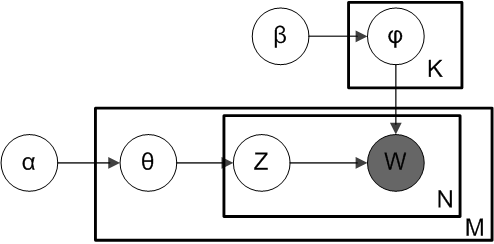
\includegraphics[width=0.5\linewidth]{fig/Smoothed_LDA}
	\caption{This is the plate representation of LDA. $\alpha$ and $\beta$ are the parameters of the two Dirichlet distributions from which are drawn, respectively, the parameters of a document-specific categorical distribution of topics and a topic-specific categorical distribution of words. Given these two distribution the process is analogue to PLSA. \\ By Slxu.public - Own work, CC BY-SA 3.0, \url{https://commons.wikimedia.org/w/index.php?curid=7922733}}
	\label{fig:smoothedlda}
\end{figure}

We call $\alpha$ the $K$-vector of the parameters of the Dirichlet distribution from which are drawn the parameters of a document-specific categorical distribution of topics $\theta_{dk}$ and $\beta$ the $W$-vector of the parameters of the Dirichlet distribution from which are drawn the parameters of a topic-specific categorical distribution of words $\phi_{kw}$. LDA can be symmetric with respect to $\alpha$ or $\beta$ if all the elements of the vector have the same value or asymmetric if the vector is allowed to have different values for each element. \textcite{wallach2009} have argued in favour of having asymmetric $\alpha$ and symmetric $\beta$, while \textcite{shiNewEvaluationFramework2019} have shown the effects of the choice of $\alpha$ and $\beta$ on the sparseness of $\theta$ and $\phi$.

LDA is a parametric algorithm, and the same considerations made for PLSA on how to determine $K$ still apply.

To infer an LDA model there are two possibilities. 
The first is to use the EM-like algorithm (also called Variation Bayes - VB) introduced by \textcite{blei2003} which operates similarly to the one discussed for PLSA, where the latent variables introduced split the problem in two independent parts: find the topics of each document, and generate the words in the document from the chosen topics.
The second is to use the MonteCarlo - Markov Chain (MCMC) algorithm introduced by \textcite{griffiths2004} (based on the Gibbs' sampling scheme - GS) in which the estimations of $\theta$ and $\phi$ are progressively improved by iterating over each word in the corpus and assigning this word to a topic with a probability estimated on the words previously seen in the corpus. 
For both these algorithms a parallel version has been developed and for the variational one also an online one (i.e. one document at time) is available \parencite{newman2009,hoffman2010}.

LDA is currently the most used algorithm, for its simplicity and speed. Moreover, a lot of different domain specific adaptations have been proposed \parencite{jelodar2019}.

On the other hand, its critics highlight two limits: the first is the absence of experimental data to support the choice of the Dirichlet priors, which additionally prevent the algorithm to be able to fit exactly a word distribution following the Zipf's law \parencite{zipf1965} (i.e. a power law or Pareto distribution of the absolute frequencies) \parencite{gerlach2018}; the second is it being a parametric model, but a non-parametric adaptation will be introduced in the next section.

\section{Hierarchical Dirichlet Process}
We now describe a first non-parametric model, which can be interpreted as an extension of LDA.

To explain the logic behind the Hierarchical Dirichlet Process (HDP) algorithm \parencite{teh2005}, it is useful to introduce the Dirichlet Process (DP).

Following \textcite{teh2005} a DP can be modelled with the so-called \textit{P\'{o}lya urn scheme} ``\textit{in which a ball of a
distinct color is associated with each [category]. The balls are drawn equiprobably; when a ball is drawn it is placed back in the urn together with another ball of the same color. In addition, with probability proportional to $\alpha_0$ a new [category] is created by drawing from [a given distribution] and a ball of a new color is added to the urn.}''. In our context we can use the urn for a single document, the categories for the topics and the balls for the words.

We now have to extend this process to a corpus of documents, and it can be done by concatenating an outer DP which determines the topics (categories), their number and the distribution from which they are drawn, and an inner DP which assigns each word of a document to a topic.
This construction allows to share information (the number and the composition of the topics) among otherwise unrelated stochastic generative processes.

As for LDA, also for HDP a Gibbs' sampling and a variational inference algorithms are available \parencite{teh2005,wang2011,newman2009}.

\chapter{Network-based methods}
\label{ch:net}
The count matrix as defined in section \ref{sec:count} represents also the incidence matrix of a bipartite weighted network\footnote{Network theory and graph theory are very similar fields of research even if they were born in different research communities. But the two different lexicons are still both used: a graph is composed of vertexes and edges, while a network of nodes and links. For the practical use the terms are perfectly exchangeable, we have tried to not mix too much the two lexicons, preferring the network one.}\footnote{\label{fn:adj}A weighted undirected bipartite graph can be represented by a matrix in which to each vertex of the first group is assigned a row and to each vertex of the second group is assigned a column and the entries of the matrix are the weight. If we call $C$ this matrix we can obtain the full adjacency matrix, using the block notation, as $A = \left(
	\begin{array}{cc}
		0 & C \\ C^T & 0
	\end{array}
\right)$ where the vertexes are numbered following the order of the first partition and then continuing with the second.} in which the nodes represent the words and the documents, and the links and their weights represent the occurrences of each word in each document\footnote{Sometimes in literature a graph whose edges are weighted and their weights are natural numbers which can be interpreted as counts, like in our case, is called multi-graph and the weighted edges are substitute with an equal number of unweighted edges between the same couple of nodes}.

\begin{figure}[!bp]
	\centering
	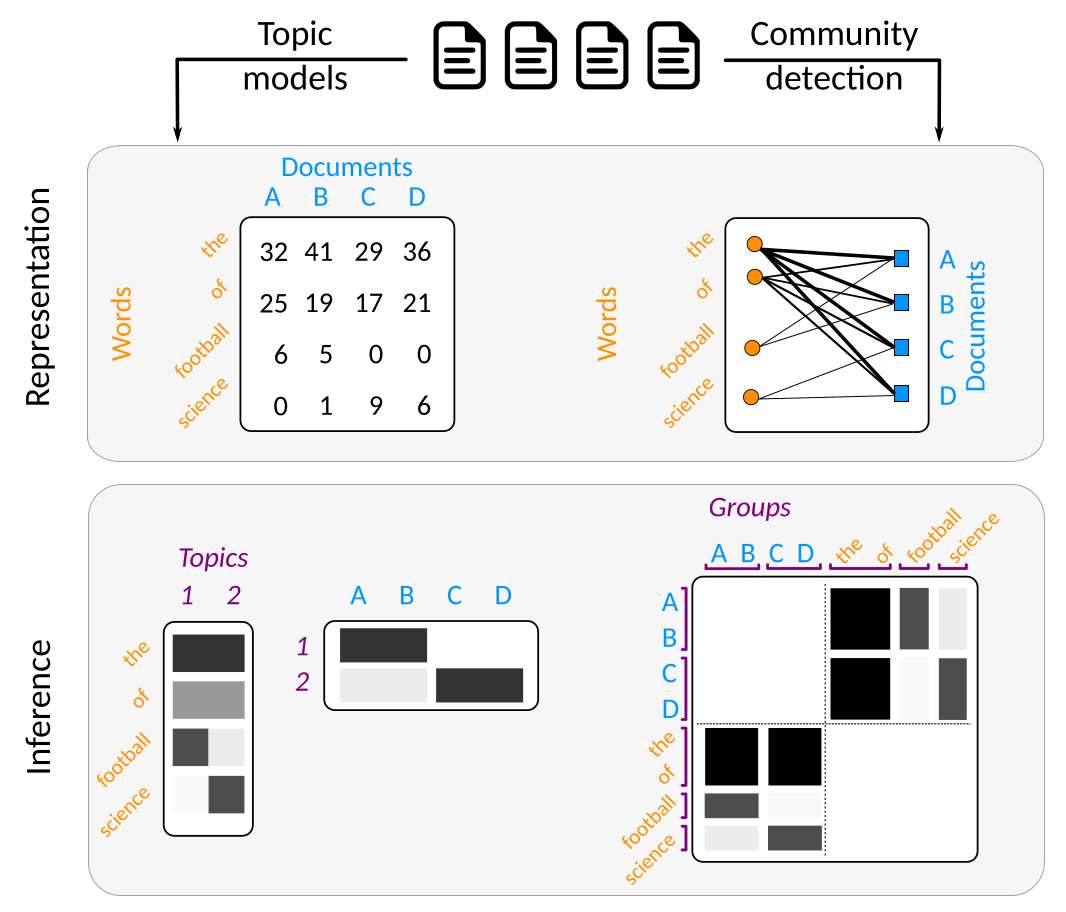
\includegraphics[width=0.5\linewidth]{fig/hsbm}
	\caption{This figure taken from \textcite{gerlach2018} illustrates very clearly the duality between the matrix representation in terms of frequencies and the graph representation. The second row of the figure represents on the left a NMF (see section \ref{sec:nmf}) decomposition, while on the right the SBM (see section \ref{sec:hsbm}) decomposition of the graph obtained from the adjacency matrix $A$ (see footnote \ref{fn:adj}).}
	\label{fig:hsbm}
\end{figure}

This representation allows to transfer the algorithm developed for community detection to the domain of Topic Models with two constrains: first, each cluster must contain either words or documents and not both (which would be the meaning of a cluster of words and documents?) and only few community detection algorithms deal well with bipartite graphs; second, we are interested in soft-cluster algorithms which assign each node to a cluster with a given probability, but many community detection algorithms perform hard-clustering assigning each node to one and one only cluster.

We have already cited in section \ref{sec:nmf} that NMF can be interpreted as the soft-clustering of a bi-partite graph, but its performance is rather poor.

Two are the possibilities: finding a representation of the corpus suitable to be hard-clustered and then recover a soft-cluster classification (like in section \ref{sec:tm} \parencite{lancichinetti2015}, \cite{kido2016} or \cite{rao2021}); using a soft-clustering algorithm which can deal with bipartite graphs (like in section \ref{sec:hsbm} \parencite{gerlach2018}); 

Both the two methods we present in this section are non-parametric, as many clustering algorithms.

\section{Topic Mapping}
\label{sec:tm}
Developing Topic Mapping, \textcite{lancichinetti2015} followed the way of translating the Topic Model problem in a hard-clustering problem and then processing the result to a soft-clustering model.

In our setting a topic is a group of words which frequently appear together. So, if we can find a way to get a new network composed only by words, whose links are weighted according to the co-occurrences of each couple of words, the communities detected in it can represent a topic.

In fact the first step of the Topic Mapping algorithm is the projection of the bipartite network in a words-only network using as weight of the links the cosine similarity between the distributions among the documents of each couple of words. If two words do not co-appear in any document their cosine similarity is 0 and the link is dropped. Then the obtained graph is compared with a null model in which the words are shuffled among all the documents: the distribution of the weights in the null model is well approximated by a Poisson distribution and only the links with a very implausible weight in the null model (i.e. with a low p-value) are kept.

The graph obtained is clustered using InfoMap \parencite{rosvall2008,rosvall2009}, which is a hard-clustering algorithm which uses an information theory approach trying to minimize the information required to describe the graph\footnote{``\textit{In order to effectively and concisely describe where on the network a random walker is, an
effective encoding of position will necessarily exploit the regularities in patterns of movement
on that network. If we can find an optimal code for describing places traced by a path on a
		network, we have also solved the dual problem of finding the important structural features of
that network. Therefore, we look for a way to assign codewords to nodes that is efficient with
respect to the dynamics on the network.}'' \parencite{rosvall2009}, where the regularities are in fact the clusters of the network.}. Finally, the clusters with less than a given number of nodes are dropped.

A soft-clustering partition in $K$ classes is a point of the $K-1$ dimensional simplex, but the vertexes of the simplex represent the certainty in the assignment, which is what the result of a hard-clustering algorithm is from the point of view of a soft-clustering algorithm. Then it is possible to encode the topics found with InfoMap as a topic-word matrix with a single one in each column to represent the cluster (topic) to which the word was assigned, and the other elements equal to zero. This matrix is used as starting point for a PLSA-like model\footnote{The process used differs substantially from that illustrated in section \ref{sec:plsa}, but still aims to get a better decomposition in the form $\mathbb{P}(w|d) = \sum_k \mathbb{P}(k|d) \mathbb{P}(w|k)$ than the one obtained with Infomap. The exact implementation is well explained in the supplementary materials of \textcite{lancichinetti2015}.} which is further refined using the LDA variational algorithm.

This algorithm can be parallelized except for the InfoMap clustering which is a sequential process\footnote{A parallel adaptation of InfoMap is available but it does not achieve the same accuracy and reproducibility \parencite{zeng2018}.}. A parallelized version of the algorithm is not straightforwardly available, even excluding the clustering step.

\section{Hierarchical Stochastic Block Model}
\label{sec:hsbm}
The Hierarchical Stochastic Block Model algorithm (hSBM) \parencite{gerlach2018} is an extension of the Stochastic Block Model algorithm (SBM) proposed by \textcite{ball2011}. 

SBM hypothesizes that in a network with $K$ communities (with $K$ a-priori fixed) each node $i$ has a probability $\theta_{ik}$ to link to another node in the community $k$, and so the probability to observe a link between the nodes $i$ and $j$ is $\sum_k \theta_{ik} \theta_{jk}$. If each node has a strong probability to belong to a few communities we can reorder the row of the adjacency matrix (and so the column given its symmetry) to observe some blocks with a high density of zero (the unrealized links among nodes of different communities) and some blocks with a high density of non-zeros values (the communities).

SBM applied to the count matrix is equivalent to PLSA \parencite{gerlach2018} if only the words are clustered, getting the topics as blocks of words.

hSBM extends SBM by explicitly accounting for the bipartite nature of the network and at the same time creating word-only and document-only clusters. 

This representation is substantially different from those we have seen until here: the other models all hypothesize that a topic can be defined as a mixture of words, and the goal is to find those mixtures and reconstruct, based on the likelihood, which of those is the more present (or in which measure each of those is present) in a document; hSBM hypothesizes that a topic is more generally what is common among similar documents (in terms of their words' composition) and that, at the same time, we can find semantically sound groups of words which often occur together.

This changes the way to characterize the topics in terms of groups of words: we can say that while other models describe a document as a mixture of mixtures of words, hSBM describes a document as a mixture of mixtures of mixtures of words. This further level of abstraction allows hSBM to capture richer and more complex topics (on the documents side) and to recognize groups of functionally similar words, for example words that are uninformative because present in every topic, which is the very definition of stopwords given in section ~\ref{sec:sw}.

Moreover, hSBM infers a hierarchy of SBMs where the communities can be merged and split among the different levels \parencite{peixoto2019} (getting in this way a non-parametric model) and relaxes the hypothesis of SBM \parencite{gerlach2018}, being able for example to fit a Zipf's distribution of words' frequencies, differently from LDA (see section \ref{sec:lda}).

The model is inferred by using a MCMC algorithm since it translates a network-theory problem in a probabilistic Bayesian one.

It is important to highlight that a hSBM is in fact a collection of models with different levels of resolution, one for each level of the hierarchy: this can be interpreted as the ability to classify, for example, documents from different disciplines and, inside each of them, recognize the different fields of research and, again, for each of them the single research topics.

\chapter{Models for corpora with metadata}
We conclude this section illustrating a recent development of the Topic Modelling problem.

It is very common to have available not only the text of the documents in a corpus but also some complementary data (generally called metadata) such as the authors, the year of publication, hyper-textual links or the citation graph which links the documents together. 

The network approach is well suited to be extended by using the concept of multi-layer network, which is a network with a single set of nodes (eventually parted in different groups which represent different entities, like words, documents, authors) but many sets of edges (eventually weighted) each representing a different aspect we want to study \parencite{hyland2021}. 

On the other hand, also a probabilistic approach based on a stochastic generative process like LDA can be enhanced to account for the information coming from metadata \parencite{rabinovich2014}.

Finally, we briefly focus on a particular kind of metadata: time. It is a common situation, for example in history of ideas, to be interested in describing how a textual corpus evolves through time.

Three are the possibilities to tackle this specific problem. The first is to infer a topic model without accounting for time and then using other statistical tools (like a regression) to explore the (cor)relations between time and topics, for example averaging the topic distribution of all the documents in a given year or considering the fraction of documents in a given year with a given topic as the most probable. The second is to develop an algorithm which includes this ordinal information and is able to describe the evolution of topics through time \parencite[e.g.][]{bleiDynamicTopicModels2006}. The last is to divide the corpus in sub-corpora each covering a smaller timespan (overlapping or not) and then finding a way to link the topics coming from different timespans: this kind of problem is studied both in the Topic Model community \parencite[e.g.][]{dicaroBimodalNetworkApproach2017} and in the community detection (a subfield of network theory) one \parencite[e.g.][]{rosvall2010}.

\chapter{Compare Topic Models}
In the first part we described some algorithms to infer a Topic Model, but we have not provided a clear criterion of choice. In fact a consensus in literature on which is the best suited algorithm for different situations, is still to be reached.

Moreover, there is no consensus on how to compare different topic models or to asses their goodness.
For probabilistic models the likelihood of the model can be a guide, but it suffers from a sensitivity on the number of parameters to be inferred (see section \ref{sec:plsa}), similarly linear algebra methods can be compared by their reconstruction error.
But neither of these is a model-agnostic framework of comparison.

We can divide the techniques proposed in literature in three groups: comparison on synthetic corpora, comparison on annotated corpora, comparison of the \textit{topic coherence} of inferred models.

With \textit{topic coherence} we indicate a set of measures which aims to describe the internal coherence of the topics given a reference corpus, the one used to infer the model or a different one \parencite{roder2015}. Generally speaking this techniques take the most probable words in a topic and assess if in the reference corpus they are likely to appear in the same documents and possibly close (i.e. in the same n-gram, for small values of n). While they give insights on the likeliness of the topic inferred, they conveys little information on how well the documents are classified and heavily depend on the corpus chosen to calculate the metric. However, this kind of assessment does not require a human-classification of the original corpus, making it the only possible choice in an unsupervised setting.

A synthetic corpus is a corpus generated according to a given stochastic process, for example the one hypothesized by LDA (see section \ref{sec:lda}), using symbolic tokens, like numbers, as words and assigning each document to a true mixture of topics which the model has to infer. It is very useful to asses if a model which aims to describe a stochastic process is in fact able to do that, but it is debatable which synthetic corpora are similar enough to real corpora to provide a good benchmark. An example of benchmark realized with this technique is presented in \textcite{shiNewEvaluationFramework2019}.

The last strategy requires a classified corpus to be available. Some corpora are relatively easy to be obtained with a classification, for example documents written in different languages, documents retrieved by organized collections like Wikipedia, Scopus or Web of Science, messages sent in similar but theme-specific newsgroups or bulletin-board.
Some research groups have produced human-classified corpora (even at sentence levels) \parencite[e.g.][]{merzManifestoCorpusNew2016} while others have tried to extend human classification to large corpora using machine learning techniques \parencite[e.g.][]{angrist2017}.

We have chosen to follow the strategy of the comparison with annotated corpora and in the next chapters we describe how the comparison was made and the results obtained.

\section{Measures}
In the setting we have chosen, we have to assess if a model is able to classify a document in the correct group represented by the label assigned in the original corpus, comparing it with the topic assigned by the Topic Model. 

A problem with this task is that we do not know which topic better represents each label. For this reason we looked for a measure of similarity which is independent from the order in which topics and labels are listed.

Furthermore, we did not enforce that the topics inferred will be the same number of the labels, and for non-parametric models doing this is in fact impossible and meaningless, and so we need a measure which is able to compare a different number of topics and labels.

Moreover, we compared really different models, and so we needed a measure that could be easily interpreted with little to no context. Generally, normalized measures which have a maximum value (perfect match) and a minimum value (no match at all) are used in these cases.

Finally, we do not have a classification of a document in a topic, even if it can be obtained by choosing the topic with the maximum score (or probability), but rather, a distribution of probabilities to belongs to a topic. This situation is common in community detection benchmarks for soft-clustering algorithms.

A measure with all these features is the Normalized Mutual Information \parencite{vinh2010} and particularly its extension to soft-clustering \parencite{lei2014}, which allows to quantify how similar two distributions are.

We will also use this measure to compare the similarity of the predictions of two models, by using one of the two predictions in place of the labels.

\subsection{Normalized Mutual Information}
Information theory relies on the concept of entropy $H(\{p_i\}) = \sum_i p_i \log p_i$, where $\{p_i\}$ is a probability distribution.
Entropy has values in $[0,1]$ and particularly $H(\{p_i\}) = 0$ for a uniform distribution and $H(\{p_i\}) = 1$ for a degenerate distribution (i.e. with only one non-null value).
In other words, entropy is 1 when we have a certainty of the outcome (i.e. the information on the phenomenon is complete) and 0 when the is no information available on the outcome (i.e. every outcome is equiprobable).

We can try to extend the idea of entropy to a new measure which, given two probability distributions, expresses how much one helps us to describe the other, i.e. how much information on the outcomes is shared between the two distributions\footnote{In section \ref{sec:plsa} we have defined the Kullback-Lieber divergence which has some of these characteristics but it is not symmetric for the exchange of the two distributions. It is suited to compare one distribution to another and not two distributions to themself.}.
 
Calling $\mathbf{X}$ and $\mathbf{Y}$ two random variables we define the mutual information as 
\begin{align*}
	MI(\mathbf{X},\mathbf{Y}) = &\sum_{\mathbf{X},\mathbf{Y}} \mathbb{P}(\mathbf{X}\cap\mathbf{Y})\log\frac{\mathbb{P}(\mathbf{X}\cap\mathbf{Y})}{\mathbb{P}(\mathbf{X})\mathbb{P}(\mathbf{Y})} \\
	= &-\sum_{\mathbf{X},\mathbf{Y}} \mathbb{P}(\mathbf{X}\cap\mathbf{Y})\log\left(\mathbb{P}(\mathbf{X})\mathbb{P}(\mathbf{Y})\right) + \sum_{\mathbf{X},\mathbf{Y}} \mathbb{P}(\mathbf{X}\cap\mathbf{Y})\log{\mathbb{P}(\mathbf{X}\cap\mathbf{Y})} \\
	= &-\sum_{\mathbf{X},\mathbf{Y}} \mathbb{P}(\mathbf{X}\cap\mathbf{Y})\log\left(\mathbb{P}(\mathbf{X})\mathbb{P}(\mathbf{Y})\right) - H(\mathbf{X} \cap \mathbf{Y})
\end{align*}
which is (a weighted average of) the logarithm of the ratio between the observed joint distribution and the hypothetical joint distribution if the two random variables were independent, using the marginal distributions as true distributions. Note that this definition is symmetric with regard to the exchange of the two random variables.

Particularly, if two random variables are independent, which means that we cannot get any information on one observing the other, the ratio is equal to one and so $MI=0$. Moreover, since $\mathbb{P}(\mathbf{X}\cap\mathbf{Y}) \geq \mathbb{P}(\mathbf{X})\mathbb{P}(\mathbf{Y})$\footnote{$\mathbb{P}(X \cap Y) = \mathbb{P}(X|Y)\mathbb{P}(Y)$ and since $\mathbb{P}(X|Y)\geq\mathbb{P}(X)$ we have $\mathbb{P}(X \cap Y)\geq\mathbb{P}(X)\mathbb{P}(Y)$}, $MI\geq0$ and it can be interpreted as the information we gain knowing the joint distribution rather than the marginal ones.

This definition is not apparently superior limited, which makes it difficult to compare this measure among different models. But it is possible to show that $MI(\mathbf{X},\mathbf{Y}) \leq \min\{H(\mathbf{X}),H(\mathbf{Y})\}$\footnote{$
	\sum \mathbb{P}(\mathbf{X}\cap\mathbf{Y}) \log\frac{\mathbb{P}(\mathbf{X}\cap\mathbf{Y})}{\mathbb{P}(\mathbf{X})\mathbb{P}(\mathbf{Y})} 
	\leq \sum \mathbb{P}(\mathbf{X}) \log\frac{\mathbb{P}(\mathbf{X}\cap\mathbf{Y})}{\mathbb{P}(\mathbf{X})\mathbb{P}(\mathbf{Y})} 
	= - \sum \mathbb{P}(\mathbf{X}) \log\frac{\mathbb{P}(\mathbf{X})}{\mathbb{P}(\mathbf{X}|\mathbf{Y})}
	= - \sum \mathbb{P}(\mathbf{X}) \log \mathbb{P}(\mathbf{X}) + \sum \mathbb{P}(\mathbf{X}) \log {\mathbb{P}(\mathbf{X}|\mathbf{Y})}
	= H(\mathbf{X}) + \sum \mathbb{P}(\mathbf{X}) \log {\mathbb{P}(\mathbf{X}|\mathbf{Y})}
\leq H(\mathbf{X})$ given $\log {\mathbb{P}(\mathbf{X}|\mathbf{Y})} \leq 0$. The same holds for $\mathbf{Y}$ for symmetry.} and so it is possible to normalize the mutual information to have values in $[0,1]$. Among the possible choices of normalization \parencite[see][]{vinh2010} we have chosen to define the normalized mutual information (NMI) as
$$NMI(\mathbf{X},\mathbf{Y}) = \frac{MI(\mathbf{X},\mathbf{Y})}{H(\mathbf{X}) + H(\mathbf{Y})}$$

Note that to compute $MI$ only the joint distribution of $\mathbf{X}$ and $\mathbf{Y}$ is required, from which we can compute the marginal ones.

In our case of interest, the two distributions are the number of documents which show a given topic as the most probable and the number of documents belonging to a given category, adequately normalized to sum to 1.

We are in fact interested in the so-called contingency table $T$ which is a matrix with values in $\mathbb{N}$ with dimensions the number of topics times the number of labels where each entry is the number of documents with the given labels and the given topic as the most probable.

From the contingency table (which is the non-normalized joint distribution) we can recover the marginal distributions by summing on the rows or the columns and then normalizing.

This formulation is well suited for exclusive classification, in which each document is assigned to one topic (the most probable one). We now will describe how to extend this measure to probabilistic classifications.

\subsubsection{Extension to probabilistic classification}
The contingency table $T$ with dimensions $m \times n$ can be written as $T = A_1^T B_1$ where $A_1$ and $B_1$ are two matrices with dimensions number of records (the documents in our case) and, respectively, $m$ and $n$ (the number of topics and labels) whose values are 1 if the record is assigned to the class correspondent to the column and 0 otherwise.
This is the so called one-hot representation of a classification, in which for each record is defined a vector with a single 1 for the right class and 0s for all the others.

Following \textcite{lei2014} if we substitute the matrix $A_1$ and $B_1$ with two matrices $A$ and $B$ in which the rows are the probability distributions associated to the classification (i.e. the certainty of the classification), we obtain $T' = A^T B$.
This matrix do not have an immediate interpretation but if we preserve the one hot distribution for the matrix $B$ (which in our case represents the assignment of a document to a label, which is a priori determined) $T'$ is obtained by weighting each occurrence in the contingency table with the degree of certainty we have about it before summing, while $T$ is obtained by simply counting (i.e. giving weight 1 to every record).
 
\section{Example corpora}
To realize our benchmark we chose two corpora: 20Newsgroups (a dataset of messages sent into twenty newsgroups)\footnote{\url{http://qwone.com/~jason/20Newsgroups/}, retrieved by using Scikit-Learn} and a collection of abstracts from Web of Science (WOS-46985 or wos)\footnote{\url{https://data.mendeley.com/datasets/9rw3vkcfy4/6} \parencite{kowsari2017}}. 20Newsgroups is labelled by the newsgroup (out of 20) in which each message was sent, while WOS-46985 has two levels of labels: 7 categories and 134 sub-categories.

Many other possibilities are available for further studies\footnote{A non exhaustive list includes: narrative texts from project Gutenberg labelled by their genre \parencite{gerlachStandardizedProjectGutenberg2018}, political manifestos where each sentence is classified by topic \parencite{merzManifestoCorpusNew2016}, Wikipedia articles with their categories, multilingual datasets with languages as labels}.


\clearpage
\begin{refcontext}[sorting=nyt]
	\printbibliography{}
\end{refcontext}
\end{document}